\section{Module 3. Non-stationary noise estimation}
Algorithm responsible for estimating spatially variant noise map in this application was implemented based on \cite{aja2015spatially}.
In the process implementation some changes were made in the original code in order to improve its effectiveness. The changes were then approved after tests that proved usefulness of those changes. The whole algorithm can be divided into couple of main stages:
\begin{itemize}
	\item estimation of expected value in each point in the image,
	\item substraction expected value from corrupted image and doing so getting the noise,
	\item calculation of SNR (\textit{signal to noise ratio}),
	\item introductory processing of noise,
	\item filtering,
	\item correction.
\end{itemize}
Below is the exemplary MRI image corrupted with complex noise.
\begin{figure}[H]
	\centering{}
		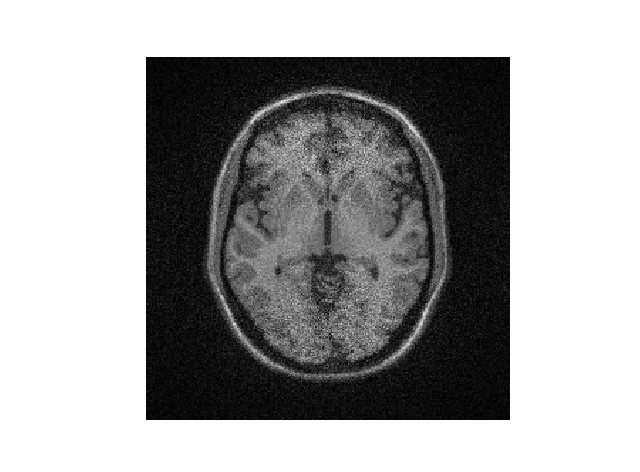
\includegraphics[scale=0.7]{figures/module03/70}
	\caption{Corrupted MRI image.} 
\end{figure}
\subsection*{Estimation of expected value in each point in the image.}
Expected value in each point of the image is estimated as a local mean using $3 x 3$ window. The local mean is calculated with the filter designed as a function called \textit{filter2b} which receives two arguments as input, first one is window, second is image.
\begin{lstlisting}[language=Python, caption = Filtering function.]
def filter2b(h,I0):

	Mx = np.size(h,1)
	My = np.size(h,0)
	Nx = (Mx-1)/2
	Ny = (My-1)/2
	Nx = int(float(Nx))
	Ny = int(float(Ny))
	It = np.pad(I0, [Nx, Ny], 'edge')
	filt = signal.convolve2d(It, np.rot90(h), mode='valid')
	return filt
\end{lstlisting}
\begin{figure}[H]
	\centering{}
		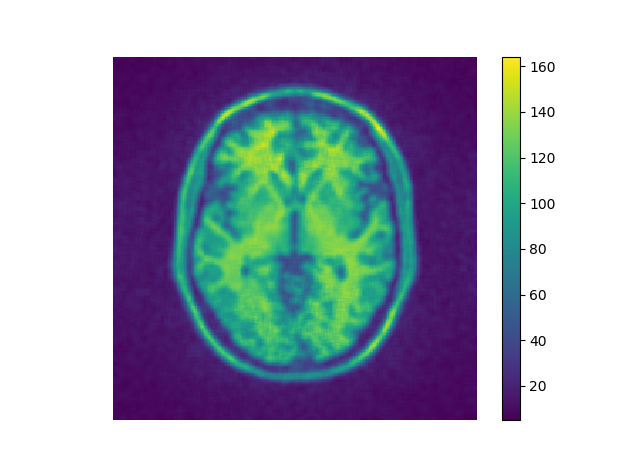
\includegraphics[scale=0.7]{figures/module03/70_local_mean}
	\caption{Local mean of image presented above.} 
\end{figure}
\subsection*{Getting the noise.}
Getting a noise from the corrupted image is accomplished by substracting local mean from the corrupted image.
\begin{figure}[H]
	\centering{}
		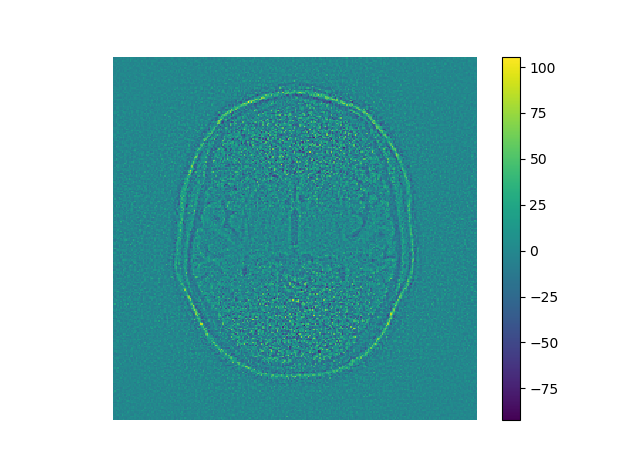
\includegraphics[scale=0.7]{figures/module03/70_szum}
	\caption{Noise.} 
\end{figure}
\subsection*{Calculation of SNR.}
This stage is more complicated than the others. Another fucntion called \textit{appro} was designed responding accordingly to the necessities of this stage. The purpose of this function is approximation of Besseli which helped during calculations of SNR.
\begin{lstlisting}[language=Python, caption = Appro.]
def appro(z):
	cont = (z<1.5)
        z8 = np.multiply(8, z)
	z8[z==0] = 0.0001
	Mn = 1 - (3/z8) - (15/2/np.power(z8, 2)) - ((3*5*21)/6/np.power(z8, 3))
	Md = 1 + (1/z8) + (9/2/np.power(z8, 2)) + ((25*9)/6/np.power(z8, 3))
	M = Mn/Md
	M = M.flatten()
	i = 0
	if(sum(sum(cont))>1):
		for x in np.nditer(z, op_flags=['readwrite']):
			if x<1.5 and x!=0:
		        x[...] = (iv(1, x))/(iv(0, x))
		    elif x==0:
			    x[...] = 0
		    else:
			    x[...] = M[i]
		    i = i +1
	return z
\end{lstlisting}
\begin{figure}[H]
	\centering{}
		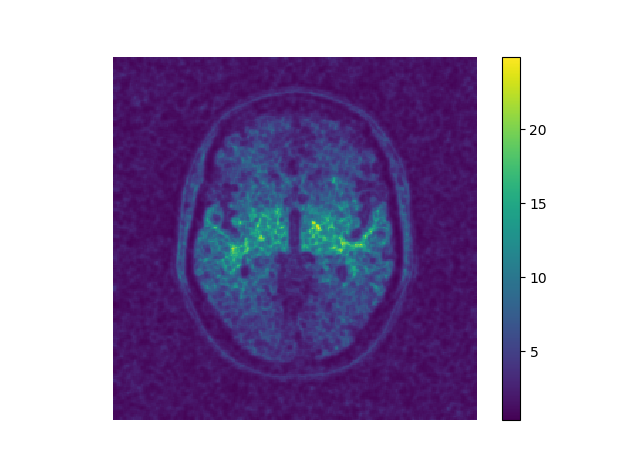
\includegraphics[scale=0.7]{figures/module03/70_snr}
	\caption{Signal to noise ratio.} 
\end{figure}
\subsection*{Indtroductory processing of noise.}
This stage cosnists of getting absolute value of each point of the noise and after that calculating logarithm of these values.
\begin{figure}[H]
	\centering{}
		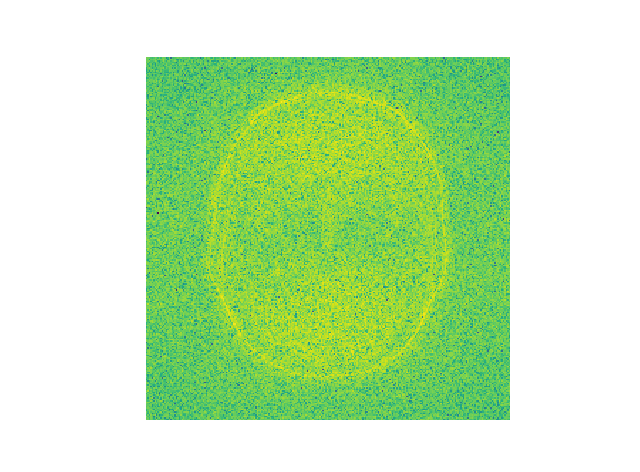
\includegraphics[scale=0.7]{figures/module03/70_log}
	\caption{Preprocessed noise.} 
\end{figure}
\subsection*{Filtering.}
Filtering occurs two times in the  alogrithm. First time after introductory processing of the noise and second time after Gaussian correction and in both cases it's low pass filtering. Filtering process is based on discrete cosine transform (\textit{dct}) and inverse discrete cosine transform (\textit{idct}), both performed in the horizontal and vertical direction. The result of \textit{dct} is matrix with the same shape as input image (in this case noise), this matrix contains frequency components of the input whith the lowest arround top-left corner. The result of \textit{dct} is muliplied by specially prepared Gaussian mask to remove high frequencies. Then the \textit{idct} of the result of this multiplication is performed to restore image from the new frequency components.
\begin{figure}[H]
	\centering{}
		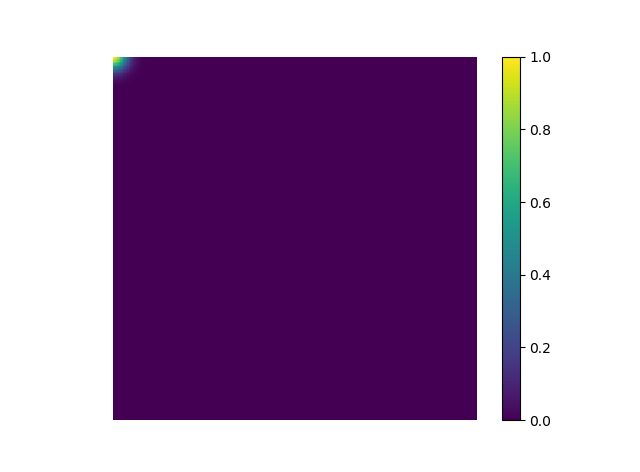
\includegraphics[scale=0.7]{figures/module03/70_gauss}
	\caption{Prepared Gaussian mask.} 
\end{figure}
\begin{figure}[H]
	\centering{}
		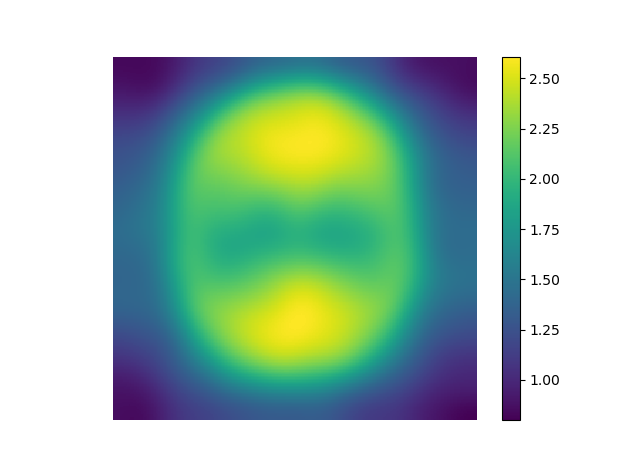
\includegraphics[scale=0.7]{figures/module03/70_lpf}
	\caption{Result of first low pass filtering.} 
\end{figure}
\subsection*{Correction.}
Correction consists of two parts. First one is Rician/Gaussian correction and second one removes residues from low pass filtering. For needs of Rician/Gaussian correction SNR was calculated earlier.
\begin{lstlisting}[language=Python, caption = Rician/Gaussian correction.]
coefs = [-0.2895, -0.0389, 0.4099, -0.3552, 0.1493, -0.0358, 0.0050, -0.00037476, 0.000011802]
correct = np.zeros((x,y)) #x and y are dimensions of the image

for i in range(0,8):
    correct = correct + np.multiply(coefs[i], np.power(SNR,i))
temp = (SNR<=2.5)
correct = np.multiply(correct, temp)
noise = noise - correct
\end{lstlisting}
\begin{figure}[H]
	\centering{}
		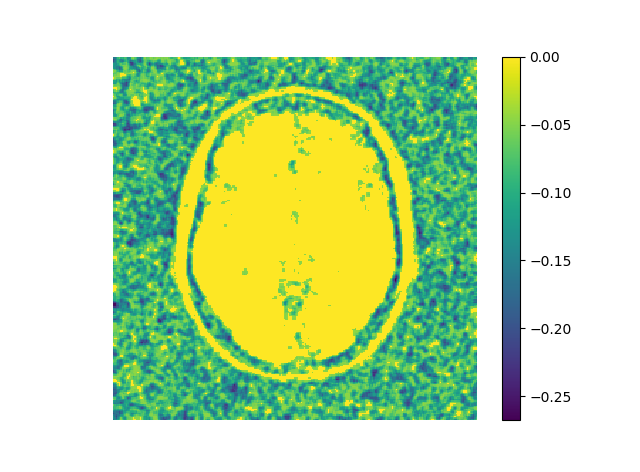
\includegraphics[scale=0.7]{figures/module03/70_korekcja}
	\caption{Correction matrix.} 
\end{figure}
\begin{figure}[H]
	\centering{}
		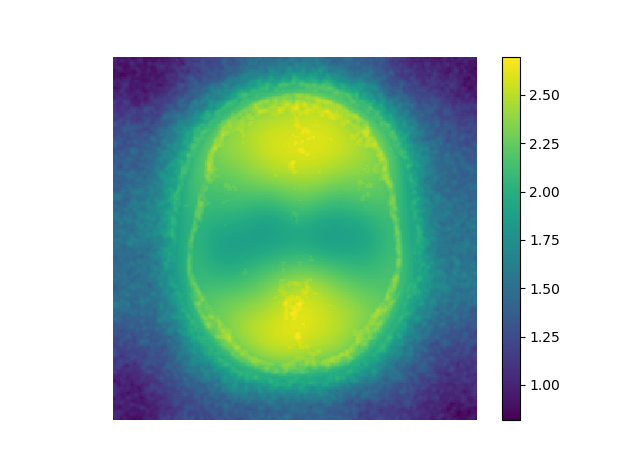
\includegraphics[scale=0.7]{figures/module03/70_I_korekcja}
	\caption{Result of Rician/Gaussian correction.} 
\end{figure}
After this part noise is filtered again with low pass filter.
\begin{figure}[H]
	\centering{}
		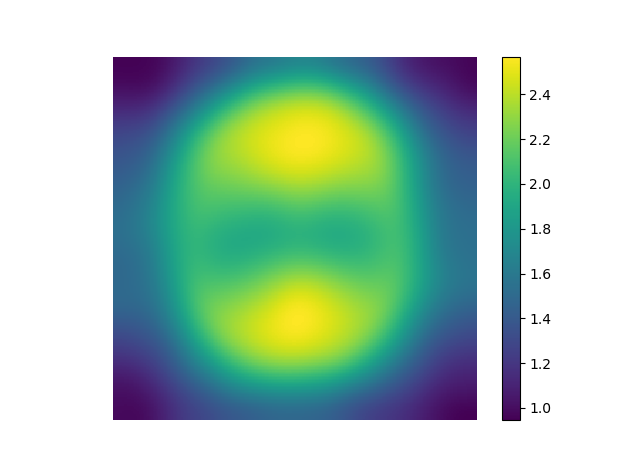
\includegraphics[scale=0.7]{figures/module03/70_lpf2}
	\caption{Result of second low pass filtering.} 
\end{figure}
In the second part of correction residues from filtering are being removed.
\begin{lstlisting}[language=Python, caption = Removing of residues from filtering.]
eg = 0.5772156649015328606/2
noise = np.multiply(2, noise)
noise /= np.sqrt(2)
temp = np.exp(eg)
noise = np.multiply(noise, temp)
\end{lstlisting}
The last part of the algorithm is getting exponential value of each point in the calculated matrix and it results in getting estimated spatially variant noise map.
\begin{figure}[H]
	\centering{}
		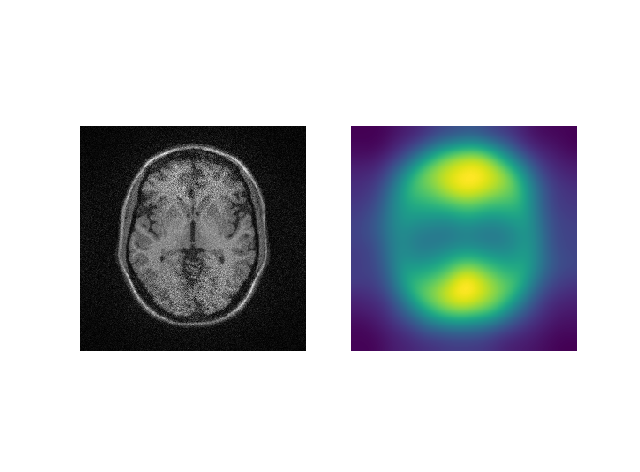
\includegraphics[scale=0.7]{figures/module03/70_zdjecie_mapa}
	\caption{Corrupted MRI image (left) with estimated map of its noise (right).} 
\end{figure}